% to turn into handout mode, add `handout` to the documentclass options
\documentclass[10pt,a4paper,handout]{beamer}
% arena_beamer.sty - shared preamble for all ARENA talk decks.
%
% Loaded BEFORE \documentclass (via plain \input, not \usepackage) so that
% it can decide whether to pass `handout` to beamer based on the \HANDOUT
% toggle. The deck pattern is:
%
%   \providecommand{\HANDOUT}{1}              % 1 = handout, 0 = presentation
%   % arena_beamer.sty - shared preamble for all ARENA talk decks.
%
% Loaded BEFORE \documentclass (via plain \input, not \usepackage) so that
% it can decide whether to pass `handout` to beamer based on the \HANDOUT
% toggle. The deck pattern is:
%
%   \providecommand{\HANDOUT}{1}              % 1 = handout, 0 = presentation
%   % arena_beamer.sty - shared preamble for all ARENA talk decks.
%
% Loaded BEFORE \documentclass (via plain \input, not \usepackage) so that
% it can decide whether to pass `handout` to beamer based on the \HANDOUT
% toggle. The deck pattern is:
%
%   \providecommand{\HANDOUT}{1}              % 1 = handout, 0 = presentation
%   \input{../../arena_beamer.sty}
%   ... deck-local macros ...
%   \begin{document} ... \end{document}
%
% CI overrides the deck's local toggle via latexmk's -usepretex flag, which
% \def's \HANDOUT before main.tex starts. The \providecommand below is a
% safety default if neither the deck nor CI set anything.

\providecommand{\HANDOUT}{1}
\ifnum\HANDOUT=1
  \PassOptionsToClass{handout}{beamer}
\fi
\documentclass[10pt,a4paper]{beamer}

\RequirePackage[latin1]{inputenc}
\RequirePackage{amsmath}
\RequirePackage{amsfonts}
\RequirePackage{amssymb}
\RequirePackage{graphicx}
\RequirePackage{ulem}
\RequirePackage{algorithm2e}
\RequirePackage{algpseudocode}
\RequirePackage{diffcoeff}
\RequirePackage{xcolor}
\RequirePackage{tikz}
\RequirePackage{cancel}
\RequirePackage{pgfplots}
\RequirePackage{background}
\RequirePackage{stmaryrd}
\RequirePackage{subcaption}
\RequirePackage{ifthen}
\RequirePackage{listings}
\RequirePackage{hyperref}

\usetheme{Madrid}

\hypersetup{
    colorlinks=true,
    linkcolor=white,
    filecolor=magenta,
    urlcolor=cyan,
}
\urlstyle{same}

\DeclareMathOperator*{\argmin}{\arg\!\min}
\DeclareMathOperator*{\argmax}{arg\,max}

\usetikzlibrary{calc, fadings, decorations.pathreplacing, automata, positioning, arrows, shapes.geometric, arrows.meta, positioning, fit, backgrounds}

% Generic math/style macros used across decks.
% Anything chapter-specific (state space, reward set, etc.) lives in the
% deck's own main.tex, not here.
\newcommand{\Ex}{\mathbb{E}}
\newcommand{\red}[1]{\textcolor{red}{#1}}
\newcommand{\bth}{{\boldsymbol{\theta}}}

% PyTorch code listing style.
\definecolor{codegreen}{rgb}{0,0.5,0}
\definecolor{codegray}{rgb}{0.4,0.4,0.4}
\definecolor{codepurple}{rgb}{0.55,0.0,0.55}
\definecolor{codeblue}{rgb}{0.0,0.0,0.6}

\lstdefinestyle{pystyle}{
    basicstyle=\ttfamily\scriptsize,
    keywordstyle=\color{codeblue}\bfseries,
    commentstyle=\color{codegreen}\itshape,
    stringstyle=\color{codepurple},
    numberstyle=\tiny\color{codegray},
    breaklines=true,
    showstringspaces=false,
    language=Python,
    morekeywords={self, nn, torch, Tensor},
    columns=fullflexible,
    keepspaces=true,
}
\lstset{style=pystyle}

% Decks set their own \graphicspath after \usepackage{arena_beamer}, but
% default to img/ so plain \includegraphics works without ceremony.
\graphicspath{{img/}}

% Falls back to a labeled placeholder box if the image file isn't present.
% Usage: \imgorplaceholder{0.6\linewidth}{filename-no-ext}{Caption shown if missing}
\newcommand{\imgorplaceholder}[3]{%
    \IfFileExists{img/#2.png}{\includegraphics[width=#1]{#2}}{%
    \IfFileExists{img/#2.jpg}{\includegraphics[width=#1]{#2}}{%
    \IfFileExists{img/#2.pdf}{\includegraphics[width=#1]{#2}}{%
    \IfFileExists{img/#2.svg}{\includegraphics[width=#1]{#2}}{%
        \fbox{\parbox[c][0.45\textheight][c]{#1}{\centering \textit{[image: #3]}\\\scriptsize drop \texttt{img/#2.(png|jpg|pdf)}}}%
    }}}}%
}

\endinput

%   ... deck-local macros ...
%   \begin{document} ... \end{document}
%
% CI overrides the deck's local toggle via latexmk's -usepretex flag, which
% \def's \HANDOUT before main.tex starts. The \providecommand below is a
% safety default if neither the deck nor CI set anything.

\providecommand{\HANDOUT}{1}
\ifnum\HANDOUT=1
  \PassOptionsToClass{handout}{beamer}
\fi
\documentclass[10pt,a4paper]{beamer}

\RequirePackage[latin1]{inputenc}
\RequirePackage{amsmath}
\RequirePackage{amsfonts}
\RequirePackage{amssymb}
\RequirePackage{graphicx}
\RequirePackage{ulem}
\RequirePackage{algorithm2e}
\RequirePackage{algpseudocode}
\RequirePackage{diffcoeff}
\RequirePackage{xcolor}
\RequirePackage{tikz}
\RequirePackage{cancel}
\RequirePackage{pgfplots}
\RequirePackage{background}
\RequirePackage{stmaryrd}
\RequirePackage{subcaption}
\RequirePackage{ifthen}
\RequirePackage{listings}
\RequirePackage{hyperref}

\usetheme{Madrid}

\hypersetup{
    colorlinks=true,
    linkcolor=white,
    filecolor=magenta,
    urlcolor=cyan,
}
\urlstyle{same}

\DeclareMathOperator*{\argmin}{\arg\!\min}
\DeclareMathOperator*{\argmax}{arg\,max}

\usetikzlibrary{calc, fadings, decorations.pathreplacing, automata, positioning, arrows, shapes.geometric, arrows.meta, positioning, fit, backgrounds}

% Generic math/style macros used across decks.
% Anything chapter-specific (state space, reward set, etc.) lives in the
% deck's own main.tex, not here.
\newcommand{\Ex}{\mathbb{E}}
\newcommand{\red}[1]{\textcolor{red}{#1}}
\newcommand{\bth}{{\boldsymbol{\theta}}}

% PyTorch code listing style.
\definecolor{codegreen}{rgb}{0,0.5,0}
\definecolor{codegray}{rgb}{0.4,0.4,0.4}
\definecolor{codepurple}{rgb}{0.55,0.0,0.55}
\definecolor{codeblue}{rgb}{0.0,0.0,0.6}

\lstdefinestyle{pystyle}{
    basicstyle=\ttfamily\scriptsize,
    keywordstyle=\color{codeblue}\bfseries,
    commentstyle=\color{codegreen}\itshape,
    stringstyle=\color{codepurple},
    numberstyle=\tiny\color{codegray},
    breaklines=true,
    showstringspaces=false,
    language=Python,
    morekeywords={self, nn, torch, Tensor},
    columns=fullflexible,
    keepspaces=true,
}
\lstset{style=pystyle}

% Decks set their own \graphicspath after \usepackage{arena_beamer}, but
% default to img/ so plain \includegraphics works without ceremony.
\graphicspath{{img/}}

% Falls back to a labeled placeholder box if the image file isn't present.
% Usage: \imgorplaceholder{0.6\linewidth}{filename-no-ext}{Caption shown if missing}
\newcommand{\imgorplaceholder}[3]{%
    \IfFileExists{img/#2.png}{\includegraphics[width=#1]{#2}}{%
    \IfFileExists{img/#2.jpg}{\includegraphics[width=#1]{#2}}{%
    \IfFileExists{img/#2.pdf}{\includegraphics[width=#1]{#2}}{%
    \IfFileExists{img/#2.svg}{\includegraphics[width=#1]{#2}}{%
        \fbox{\parbox[c][0.45\textheight][c]{#1}{\centering \textit{[image: #3]}\\\scriptsize drop \texttt{img/#2.(png|jpg|pdf)}}}%
    }}}}%
}

\endinput

%   ... deck-local macros ...
%   \begin{document} ... \end{document}
%
% CI overrides the deck's local toggle via latexmk's -usepretex flag, which
% \def's \HANDOUT before main.tex starts. The \providecommand below is a
% safety default if neither the deck nor CI set anything.

\providecommand{\HANDOUT}{1}
\ifnum\HANDOUT=1
  \PassOptionsToClass{handout}{beamer}
\fi
\documentclass[10pt,a4paper]{beamer}

\RequirePackage[latin1]{inputenc}
\RequirePackage{amsmath}
\RequirePackage{amsfonts}
\RequirePackage{amssymb}
\RequirePackage{graphicx}
\RequirePackage{ulem}
\RequirePackage{algorithm2e}
\RequirePackage{algpseudocode}
\RequirePackage{diffcoeff}
\RequirePackage{xcolor}
\RequirePackage{tikz}
\RequirePackage{cancel}
\RequirePackage{pgfplots}
\RequirePackage{background}
\RequirePackage{stmaryrd}
\RequirePackage{subcaption}
\RequirePackage{ifthen}
\RequirePackage{listings}
\RequirePackage{hyperref}

\usetheme{Madrid}

\hypersetup{
    colorlinks=true,
    linkcolor=white,
    filecolor=magenta,
    urlcolor=cyan,
}
\urlstyle{same}

\DeclareMathOperator*{\argmin}{\arg\!\min}
\DeclareMathOperator*{\argmax}{arg\,max}

\usetikzlibrary{calc, fadings, decorations.pathreplacing, automata, positioning, arrows, shapes.geometric, arrows.meta, positioning, fit, backgrounds}

% Generic math/style macros used across decks.
% Anything chapter-specific (state space, reward set, etc.) lives in the
% deck's own main.tex, not here.
\newcommand{\Ex}{\mathbb{E}}
\newcommand{\red}[1]{\textcolor{red}{#1}}
\newcommand{\bth}{{\boldsymbol{\theta}}}

% PyTorch code listing style.
\definecolor{codegreen}{rgb}{0,0.5,0}
\definecolor{codegray}{rgb}{0.4,0.4,0.4}
\definecolor{codepurple}{rgb}{0.55,0.0,0.55}
\definecolor{codeblue}{rgb}{0.0,0.0,0.6}

\lstdefinestyle{pystyle}{
    basicstyle=\ttfamily\scriptsize,
    keywordstyle=\color{codeblue}\bfseries,
    commentstyle=\color{codegreen}\itshape,
    stringstyle=\color{codepurple},
    numberstyle=\tiny\color{codegray},
    breaklines=true,
    showstringspaces=false,
    language=Python,
    morekeywords={self, nn, torch, Tensor},
    columns=fullflexible,
    keepspaces=true,
}
\lstset{style=pystyle}

% Decks set their own \graphicspath after \usepackage{arena_beamer}, but
% default to img/ so plain \includegraphics works without ceremony.
\graphicspath{{img/}}

% Falls back to a labeled placeholder box if the image file isn't present.
% Usage: \imgorplaceholder{0.6\linewidth}{filename-no-ext}{Caption shown if missing}
\newcommand{\imgorplaceholder}[3]{%
    \IfFileExists{img/#2.png}{\includegraphics[width=#1]{#2}}{%
    \IfFileExists{img/#2.jpg}{\includegraphics[width=#1]{#2}}{%
    \IfFileExists{img/#2.pdf}{\includegraphics[width=#1]{#2}}{%
    \IfFileExists{img/#2.svg}{\includegraphics[width=#1]{#2}}{%
        \fbox{\parbox[c][0.45\textheight][c]{#1}{\centering \textit{[image: #3]}\\\scriptsize drop \texttt{img/#2.(png|jpg|pdf)}}}%
    }}}}%
}

\endinput


\begin{document}

\title[{[0.2] CNNs and ResNets}]
{{[0.2] CNNs and ResNets}}

\author[David Quarel]
{David Quarel}

\institute[ARENA]
{
  ARENA
}

\date[\today]
{\today}

\frame{\titlepage}

% ------------------------------------------------------------
\begin{frame}
\frametitle{What's today about?}
\begin{itemize}
    \item Goal: by the end of today you will have built \textbf{ResNet34} from raw
    PyTorch primitives, loaded pretrained weights, and used it for transfer learning.
    \pause
    \item The road there:
    \begin{enumerate}
        \item Layers as \texttt{nn.Module}s --- the LEGO bricks.
        \pause
        \item Assemble a multi-layer perceptron, train it on MNIST.
        \pause
        \item Convolutions: a much better prior for images.
        \pause
        \item Skip connections + batch norm $\Rightarrow$ ResNet.
        \pause
        \item Feature extraction: stand on the shoulders of pretrained giants.
    \end{enumerate}
    % \pause
    % \item Theme: \textit{build the primitives yourself}, so the rest of the program
    % is never a black box.
\end{itemize}
\end{frame}

% ------------------------------------------------------------
\begin{frame}
\frametitle{Why deep learning?}
\begin{itemize}
    \item Classical ML: hand-engineer features,
    learn a thin classifier on top.
    \pause
    \item Deep learning: \textit{learn the features too}, end-to-end, from raw data.
    \pause
    \item \textbf{Universal approximation:} a sufficiently wide MLP with a
    nonlinearity can approximate any continuous function on a compact set.
    \begin{itemize}
        \item Existence, not efficiency. Architecture priors (convolutions,
        attention, skip connections) are what make it tractable.
    \end{itemize}
    \pause
    \item Interpretability work later: knowing exactly what
    the model is made of is the prerequisite for taking it apart.
\end{itemize}
\end{frame}

% ------------------------------------------------------------
\begin{frame}[fragile]
\frametitle{The \texttt{nn.Module} pattern}
\begin{itemize}
    \item Everything in a PyTorch model is a \texttt{Module}: layers, blocks,
    the whole network. A \texttt{Module} bundles \textit{parameters} with a
    \texttt{forward} pass.
    \pause
\end{itemize}
\begin{block}{}
\begin{lstlisting}
    class Linear(nn.Module):
        def __init__(self, d_in, d_out):
            super().__init__()
            # define parameters here
            self.W = nn.Parameter(torch.randn(d_out, d_in))
            self.b = nn.Parameter(torch.zeros(d_out))

        def forward(self, x):
            # defines what the module does
            y = einsum(x, self.W, "... d_in, d_out d_in -> ... d_out") + self.b
            # equiv. y = x @ self.W.T + self.b
            return y

    >>> module = Linear(d_in=3, d_out=5)
    >>> module(x) #equiv. to module.forward(x)
\end{lstlisting}
\end{block}
\pause
\begin{itemize}
    \item \texttt{nn.Parameter} $\Rightarrow$ tracked by \texttt{.parameters()},
    updated by the optimizer.
    \pause
    \item Modules can nest other modules; used often today
\end{itemize}
\end{frame}

% ------------------------------------------------------------
\begin{frame}[fragile]
\frametitle{The training loop}
\begin{itemize}
    \item Same four steps every iteration: \textit{forward, loss, backward, step}.
\end{itemize}
\begin{block}{}
\begin{lstlisting}
    for x, y in dataloader:                 # sample data in batches
        y_hat = model(x)                    # forward pass through model
        loss = my_loss_function(y,y_hat)    # how good was the model?
        loss.backward()                     # compute gradient of loss w.r.t parameters
        optimizer.step()                    # update parameters to decrease loss
        optimizer.zero_grad()               # reset gradients before next batch
\end{lstlisting}
\end{block}
\pause
\begin{itemize}
    \item \texttt{loss.backward()} fills \texttt{.grad} on every parameter via
    autograd.
    \pause
    \item \texttt{optimizer.step()} applies an update rule
    (e.g.\ Adam: momentum + per-parameter adaptive learning rate).
    \pause
    \item \texttt{zero\_grad()} before backward: gradients \textbf{accumulate}
    by default in PyTorch.
\end{itemize}
\end{frame}

% ------------------------------------------------------------
\begin{frame}
\frametitle{Cross-entropy loss}
\begin{itemize}
    \item Model outputs logits $z \in \R^K$; convert to probabilities with
    softmax:
    $$ \hat{p}_k = \frac{\exp(z_k)}{\sum_j \exp(z_j)} $$
    \pause
    \item True label $y$ is one-hot. Cross-entropy:
    \begin{block}{Cross-Entropy}
        $$ \mathcal{L}(z, y) = -\sum_{k} y_k \log \hat{p}_k
        = -\log \hat{p}_{y^*} $$
    \end{block}
    where $y^*$ is the index of the true class.
    \pause
    \item PyTorch's \texttt{F.cross\_entropy} takes \textit{logits directly}
    and fuses softmax + log internally for numerical stability.
\end{itemize}
\end{frame}

% ------------------------------------------------------------
\begin{frame}
\frametitle{Why convolutions?}
\begin{itemize}
    \item A 224$\times$224 RGB image is a 150{,}528-dimensional vector.
    A fully-connected first layer with 1000 hidden units has $\sim 1.5 \times 10^8$
    parameters \emph{just} for one layer.
    \pause
    \item Images have structure that an MLP completely ignores. Convolutions bake
    in three priors:
    \begin{enumerate}
        \item \textbf{Locality:} nearby pixels are more related than distant ones.
        \pause
        \item \textbf{Translation equivariance:} a cat in the corner is still a
        cat. Same filter, applied everywhere.
        \pause
        \item \textbf{Weight sharing:} one kernel reused across all positions
        $\Rightarrow$ orders of magnitude fewer parameters.
    \end{enumerate}
    \pause
    \item Same idea, different domain: this is to images what attention is to
    sequences.
\end{itemize}
\end{frame}

% ------------------------------------------------------------
\begin{frame}
\begin{center}
    \imgorplaceholder{\linewidth}{conv2d}{Conv2d kernel sliding over input}
\end{center}
\end{frame}

% ------------------------------------------------------------
\begin{frame}
\frametitle{MaxPool}
\begin{itemize}
    \item \textbf{Pooling} downsamples a feature map; we replace each
    $k \times k$ window with its maximum:
\end{itemize}
\begin{center}
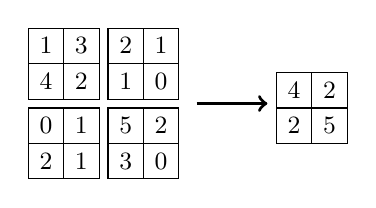
\begin{tikzpicture}[scale=0.45, every node/.style={font=\small}]
    % Input 4x4 split into four 2x2 quadrants with a small visible gap so
    % the pooling regions are obvious.
    \def\g{0.25}
    \foreach \x/\y/\v in {
        0/3/1, 1/3/3, 2/3/2, 3/3/1,
        0/2/4, 1/2/2, 2/2/1, 3/2/0,
        0/1/0, 1/1/1, 2/1/5, 3/1/2,
        0/0/2, 1/0/1, 2/0/3, 3/0/0%
    }{%
        \pgfmathsetmacro{\dx}{\x >= 2 ? \g : 0}
        \pgfmathsetmacro{\dy}{\y >= 2 ? \g : 0}
        \draw (\x+\dx, \y+\dy) rectangle (\x+1+\dx, \y+1+\dy);
        \node at (\x+0.5+\dx, \y+0.5+\dy) {\v};
    }

    % Arrow, vertically centered on the (now slightly taller) input.
    \draw[->, very thick] (4.5+\g, 2+0.5*\g) -- (6.5+\g, 2+0.5*\g);

    % Output 2x2
    \foreach \x in {0,1}
        \foreach \y in {0,1} {
            \draw (7+\x,1+\y) rectangle (8+\x,2+\y);
        }
    \node at (7.5, 2.5) {4}; \node at (8.5, 2.5) {2};
    \node at (7.5, 1.5) {2}; \node at (8.5, 1.5) {5};
\end{tikzpicture}
\end{center}
\pause
\begin{itemize}
    \item No learnable parameters. Provides small-shift invariance and shrinks
    the spatial dimensions cheaply.
    \pause
    \item Used between conv stages to gradually trade spatial resolution for
    channel depth.
\end{itemize}
\end{frame}

% ------------------------------------------------------------
\begin{frame}
\frametitle{Going deeper hurts (the degradation problem)}
\begin{itemize}
    \item Intuition: a 56-layer net should be \textit{at least} as good as a
    20-layer net: it could just learn identity in the extra layers.
    \pause
    \item Empirically, plain deep nets do \textbf{worse}, even on training data.
\end{itemize}
\begin{center}
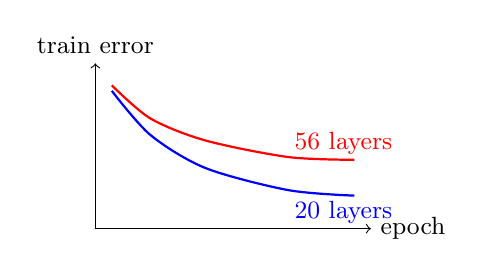
\begin{tikzpicture}[scale=0.7]
    \draw[->] (0,0) -- (5,0) node[right, font=\small] {epoch};
    \draw[->] (0,0) -- (0,3) node[above, font=\small] {train error};
    \draw[thick, blue]   plot[smooth] coordinates {(0.3, 2.5) (1, 1.7) (2, 1.1) (3.5, 0.7) (4.7, 0.6)};
    \draw[thick, red]    plot[smooth] coordinates {(0.3, 2.6) (1, 2.0) (2, 1.6) (3.5, 1.3) (4.7, 1.25)};
    \node[font=\small, blue] at (4.5, 0.3) {20 layers};
    \node[font=\small, red]  at (4.5, 1.55) {56 layers};
\end{tikzpicture}
\end{center}
\pause
\begin{itemize}
    \item Gradients struggle to propagate cleanly through many layers; identity
    is hard to \textit{learn} from scratch.
\end{itemize}
\end{frame}

% ------------------------------------------------------------
\begin{frame}
\frametitle{Skip connections (residual learning)}
\begin{itemize}
    \item \textbf{Idea:} make identity the \textit{default}. Each block learns
    a residual $F(x)$ added to its input.
\end{itemize}
\begin{block}{Residual block}
    $$ y = F(x; \theta) + x $$
\end{block}

\pause
\begin{itemize}
    \item Gradients flow back through the identity branch unimpeded.
    \pause
    \item Now training 100+ layer networks is routine.
\end{itemize}
\end{frame}

% ------------------------------------------------------------
\begin{frame}
\frametitle{Pretrained models and feature extraction}
\begin{itemize}
    \item Training ImageNet-scale models from scratch is expensive. Almost no
    one does it twice.
    \pause
    \item \textbf{Transfer learning:} take a pretrained backbone, replace the
    final classifier, train only the new head on your task.
    \begin{itemize}
        \item Freeze backbone: \texttt{p.requires\_grad = False} for every
        backbone parameter.
        \pause
        \item Swap in a fresh \texttt{Linear} sized for your new label set.
        \pause
        \item Optimizer only sees the unfrozen parameters.
    \end{itemize}
    \pause
    \item Today: take your ResNet34, freeze it, retrain the head on CIFAR-10.
    % \pause
    % \item This is the lever almost every applied DL project pulls first.
\end{itemize}
\end{frame}

% ------------------------------------------------------------
\begin{frame}
\small{
\frametitle{Glossary}
\begin{itemize}
    \item \textbf{Module} (\texttt{nn.Module}): bundle of parameters + a
    \texttt{forward}. Composable.
    \item \textbf{Parameter} vs \textbf{Buffer}: both stored in
    \texttt{state\_dict}; only Parameters get gradients.
    \item \textbf{ReLU}: $\max(0, x)$. The default nonlinearity.
    \item \textbf{Linear}: $y = Wx + b$. Kaiming-init for ReLU nets.
    \item \textbf{Cross-entropy}: $\mathcal{L} = -\log \hat{p}_{y^*}$.
    \item \textbf{Conv2d}: kernel + stride + padding sliding over spatial dims.
    \item \textbf{MaxPool}: take the max over a $k\times k$ window; no params.
    \item \textbf{BatchNorm}: normalize per channel; learned $\gamma,\beta$;
    running stats in eval mode.
    \item \textbf{Residual block}: $y = F(x) + x$. Identity is the default.
    % \item \textbf{Block group}: repeat residual blocks at a fixed resolution;
    % optionally downsample at entry.
    %\item \textbf{ResNet34}: stem $\to$ groups $(3,4,6,3)$ $\to$ GAP $\to$ FC.
    \item \textbf{Training step:} forward $\to$ loss
    $\to$ \texttt{backward} $\to$ \texttt{step} $\to$ \texttt{zero\_grad}. 
    \item \textbf{Feature extraction:} freeze backbone, train new head on a new
    task.

    \hspace{0pt}
    \rule{0.3\textwidth}{0.5pt}
    \vspace{0.1cm}

    \footnotesize{The whole point of today: build each row above yourself, so
    by the end none of it is a black box.}
\end{itemize}
}
\end{frame}

\end{document}
